\chapter{INTRODUÇÃO}
    
     O método geofísico \index{magnetotelúrico}, utiliza as baixas frequências do espectro eletromagnético, para investigar a subsuperfície do planeta Terra. A interação do vento solar com o campo magnético terrestre, compõe a origem dessas ondas eletromagnéticas.  
    
    A grande complexidade dos dados desestimula o desenvolvimento de para o processamento dos mesmos. Atualmente os programas destinados a esse tipo de atividade são proprietários,\cite{cagniard1953basic} com alto valor comercial, ou são livres operacionais exclusivamente por linhas de comando.  
    
    A comunidade MTnet, mantém laços com diversos pesquisados na área do MT, e reúne as aplicações destinadas aos processamentos, tais como:  de pré-processamento, inversão, tratamento estatísticos, dentre outros. Os programas alocados no MTnet são de uso livre e destinados a comunidade acadêmica.
    
    \begin{figure}[H]
        \caption{Modelo de Aquisição para ADU.}
        \begin{center}
         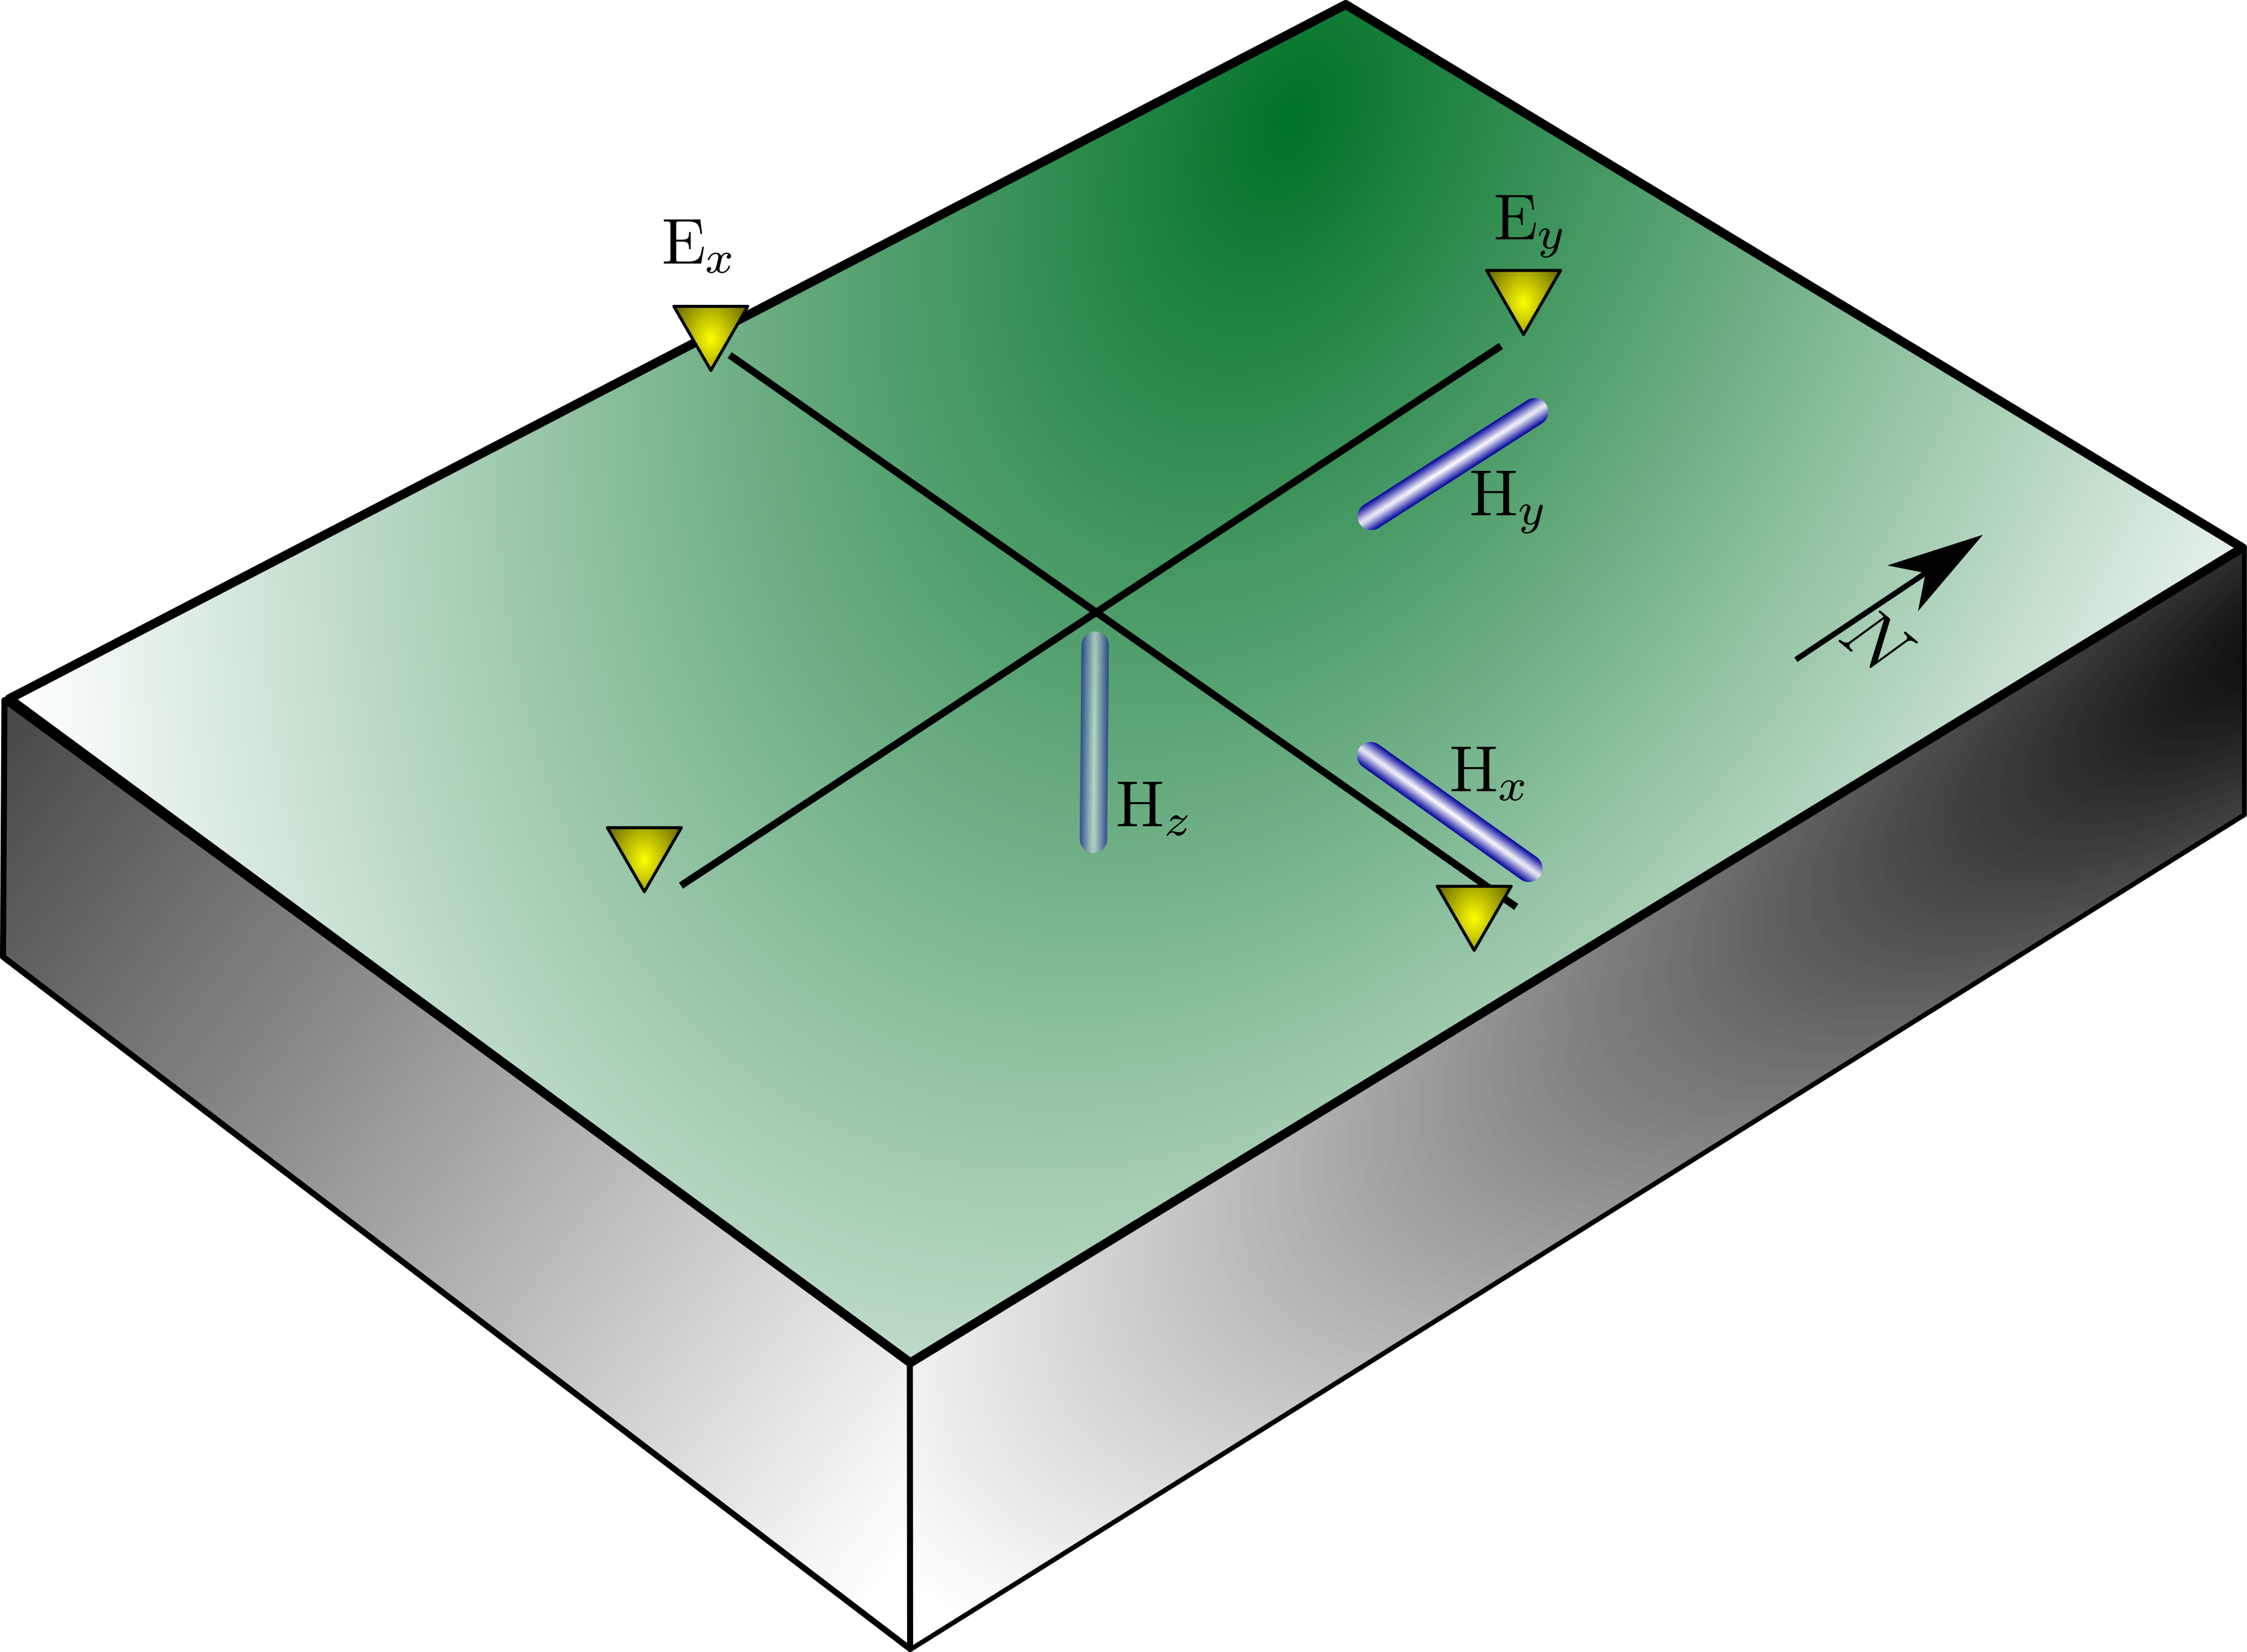
\includegraphics[width=10cm]{fig/ADU_MODELO.png}
        \end{center}
        \legend{\Fonte{\oautor}}
    \end{figure}
     O método geofísico \index{magnetotelúrico}, utiliza as baixas frequências do espectro eletromagnético, para investigar a subsuperfície do planeta Terra. A interação do vento solar com o campo magnético terrestre, compõe a origem dessas ondas eletromagnéticas.
     
     \begin{figure}[htp]
        \caption{Modelo de Aquisição para ADU}
        \begin{center}
         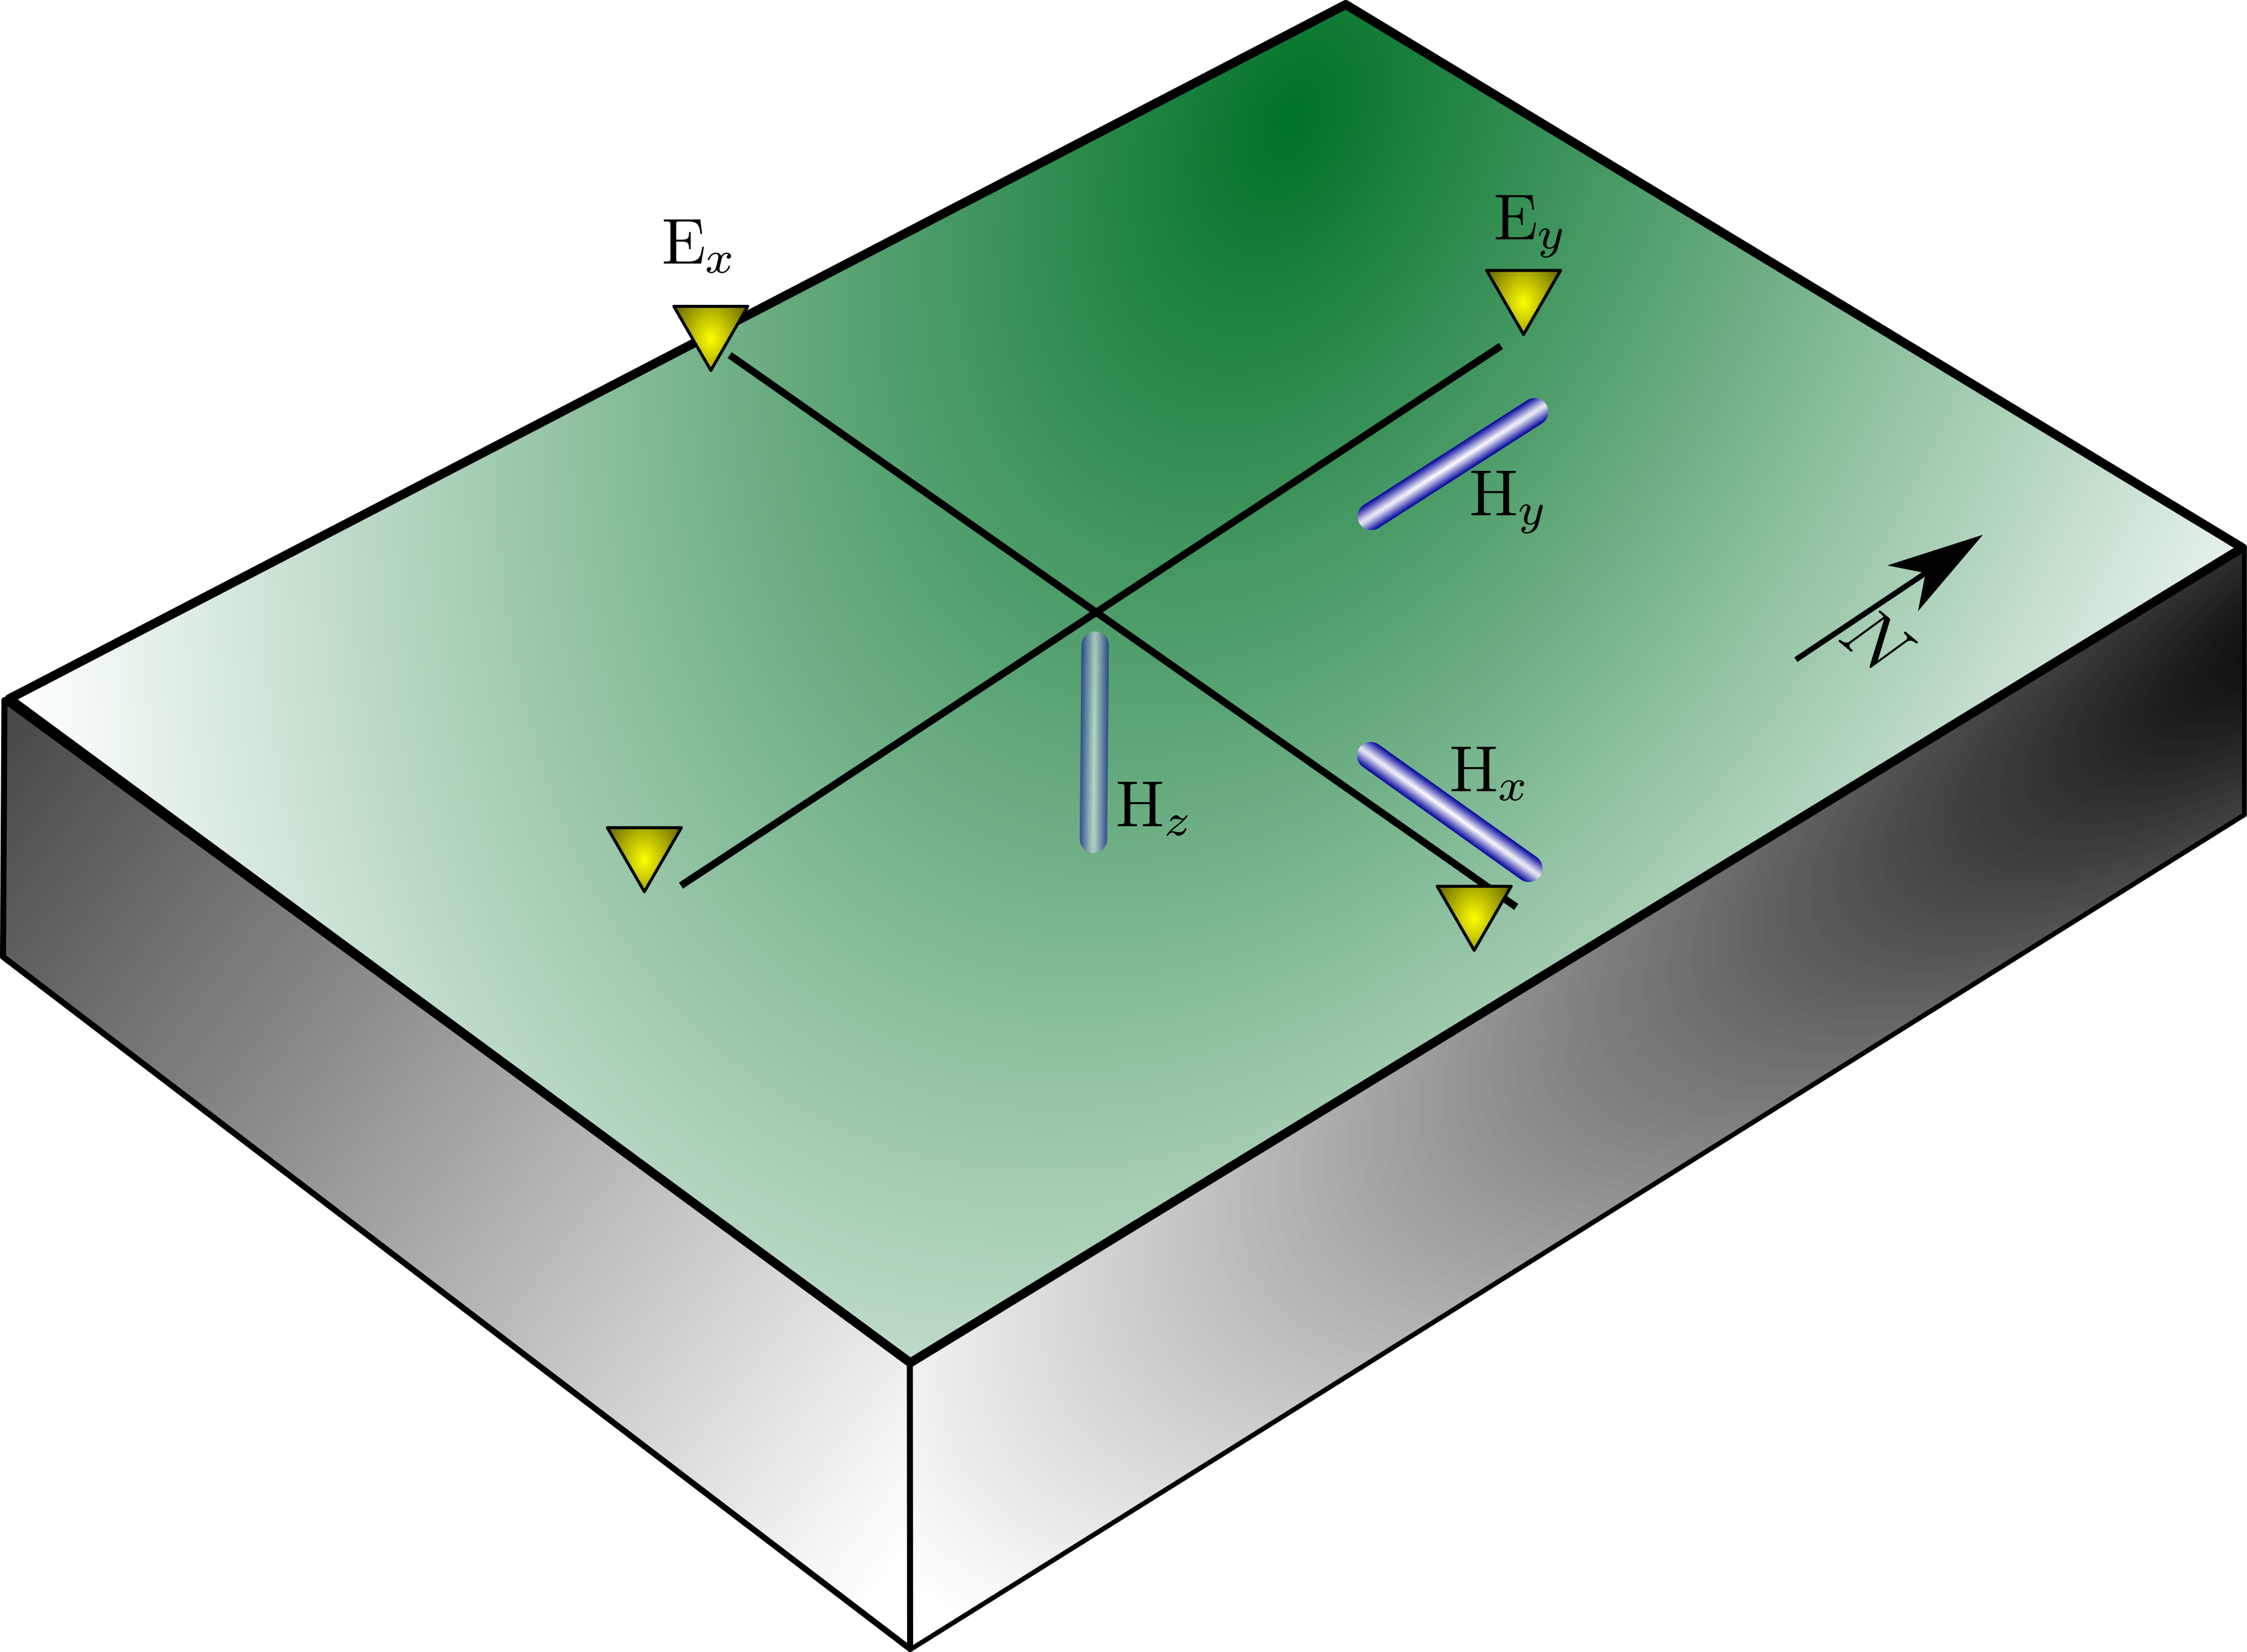
\includegraphics[width=10cm]{fig/ADU_MODELO.png}
        \end{center}
        \legend{\Fonte{\oautor}}
    \end{figure}

    \section{Uma secção}
        vamos colocar um equação beta aqui 
        
        \begin{equation}
         V = d^2
        \end{equation}
        
        vamos citar o marcelo kkkkk \cite{padua2004estudos}

    
    \subsection{Uma subsection}
    \subsubsection{UMA SUBSUSBUSBSECÇÃO}
